% Først spesifiserer vi hvilken dokumentklasse vi vil ha og noen 
% globale opsjoner. Bytt ut 'article' med 'book' hvis du vil ha 
% med kapitler.
\documentclass[a4paper, twoside, titlepage, 11pt]{article}

% Så sier vi fra om hvilke tilleggspakker vi trenger
% til dokumentet vårt. De som du ikke trenger (se kommentaren) 
% kan det være en fordel å kommentere ut (sett prosenttegn foran),
% da vil kompilering gå raskere.

\usepackage[norsk]{babel}             % norske navn rundt omkring
\usepackage[T1]{fontenc}              % norsk tegnsett (æøå)
\usepackage[latin1]{inputenc}         % norsk tegnsett
\usepackage{geometry}                 % anbefalt pakke for å styre marger.
\usepackage{datetime}
\usepackage{amsmath,amsfonts,amssymb} % matematikksymboler
\usepackage{amsthm}                   % for å lage teoremer og lignende.
\usepackage{graphicx}                 % inkludering av grafikk
\usepackage{subfig}                   % hvis du vil kunne ha flere
\usepackage{hyperref}
\usepackage{xcolor}
\usepackage{float}
% \input{preamble/preamble.tex}
% \input{preamble/preamble-addon-listings.tex}
 

                                      % figurer inni en figur
\usepackage{listingsutf8}                 % Fin for inkludering av kildekode

%\usepackage{hyperref}                % Lager hyperlinker i evt. pdf-dokument
                                      % men har noen bugs, så den er kommentert
                                      % bort her.

\usepackage{color}

\definecolor{mygreen}{rgb}{0,0.6,0}
\definecolor{mygray}{rgb}{0.5,0.5,0.5}
\definecolor{mymauve}{rgb}{0.58,0,0.82}
\lstdefinestyle{customc}{
  belowcaptionskip=1\baselineskip,
  breaklines=true,
  frame=L,
  xleftmargin=\parindent,
  language=C,
  showstringspaces=false,
  basicstyle=\footnotesize\ttfamily,
  keywordstyle=\bfseries\color{green!40!black},
  commentstyle=\itshape\color{purple!40!black},
  identifierstyle=\color{blue},
  stringstyle=\color{orange},
}    
\lstdefinestyle{customasm}{
  belowcaptionskip=1\baselineskip,
  frame=L,
  xleftmargin=\parindent,
  language=[x86masm]Assembler,
  basicstyle=\footnotesize\ttfamily,
  commentstyle=\itshape\color{purple!40!black},
}
\lstset{escapechar=@,style=customc} 

\graphicspath{{./results/}}                          
% Indeksgenerering er kommentert ut her. Ta bort prosenttegnene
% hvis du vil ha en indeks:
%\usepackage{makeidx}     
%\makeindex              

% Selve dokumentet begynner:

\begin{document}

% På forsida skal vi ikke ha noen sidenummerering:

% \pagestyle{empty}
% \pagenumbering{roman}

% Inkluder forsida:
% Enkel forside som bruker latex sin \titlepage kommando:
% NB: Bruken av \and mellom navn!
\titlepage
\title{TMA4280 - Problem set 6}
\author{Tor Holm Slettebak}
\date{\today}
\maketitle

% Local Variables:
% TeX-master: "master"
% End:

% Romerske tall på alt før selve rapporten starter er pent.
\pagenumbering{roman}

% For å ikke begynne innholdslista på baksida av forsida:
%\cleardoublepage
% (kun aktuelt når man har twoside som global opsjon)

% Nå vi vil ha noe i topp- og bunnteksten
\pagestyle{headings}

% Si til LaTeX at vi vil ha ei innholdsliste generert akkurat her:
%\tableofcontents

% Pass på at neste side ikke begynner på baksida av en annen side.
%\cleardoublepage

% Arabisk (vanlige tall) sidenummerering. Starter på side 1 igjen.
\pagenumbering{arabic}

% Inkluder alle de andre kildefilene:

% NB: Vi trenger ikke ta med filendelsen .tex her. Den vet
%     LaTeX om selv!



\section{The poisson program}
In the beginning I tried to take advantage of our professors framework of several poisson solvers, which uses vectors and matrices in Fortran format. This however turned out to be hard for me. When I tried to create a transpose operation in parallel I could not make it work. So I made a switched to the code distributed with the problemtext, which is written by Einar M. Rønquist. 

\section{Parallelization}
To parallelize the problem I chose to split up the problem in lesser parts, each solvable by it self. Each process generates it own matrix B, and modifies it through the program, before it shares it result with each of the other processes and the maximal error is calculated. During each process' execution the only communication, except for in assembly, between the threads are done in the transpose operation.

\subsection{The transpose operation}
Since each process has a part of the matrix b, a transpose will need to swap elements with other processes. This communcation is done through MPI\_Alltoallv (see figure \ref{fig:transpose}), a MPI call which sends a sendarray according to a count array and a displacement array. The countarray contains the number of elements to be sent to each process. The displacement arrays entry i specifies the displacement relative to the sendarray, entry i is sent to process i. The receive buffer is filled according to the same displacement and count array. 

During the writing of this report, and after results had been obtained, I found that I had created a duplicate matrixAsVec operation. In the transpose operation I believe a less effective version of this has been used, a version not using memcpy(). This may have some small effect on runtime, but no real testing has been performed to confirm this.

% Here insert the illustration of alltoallv from problem text.
\begin{figure}[htbp]
	\centering
	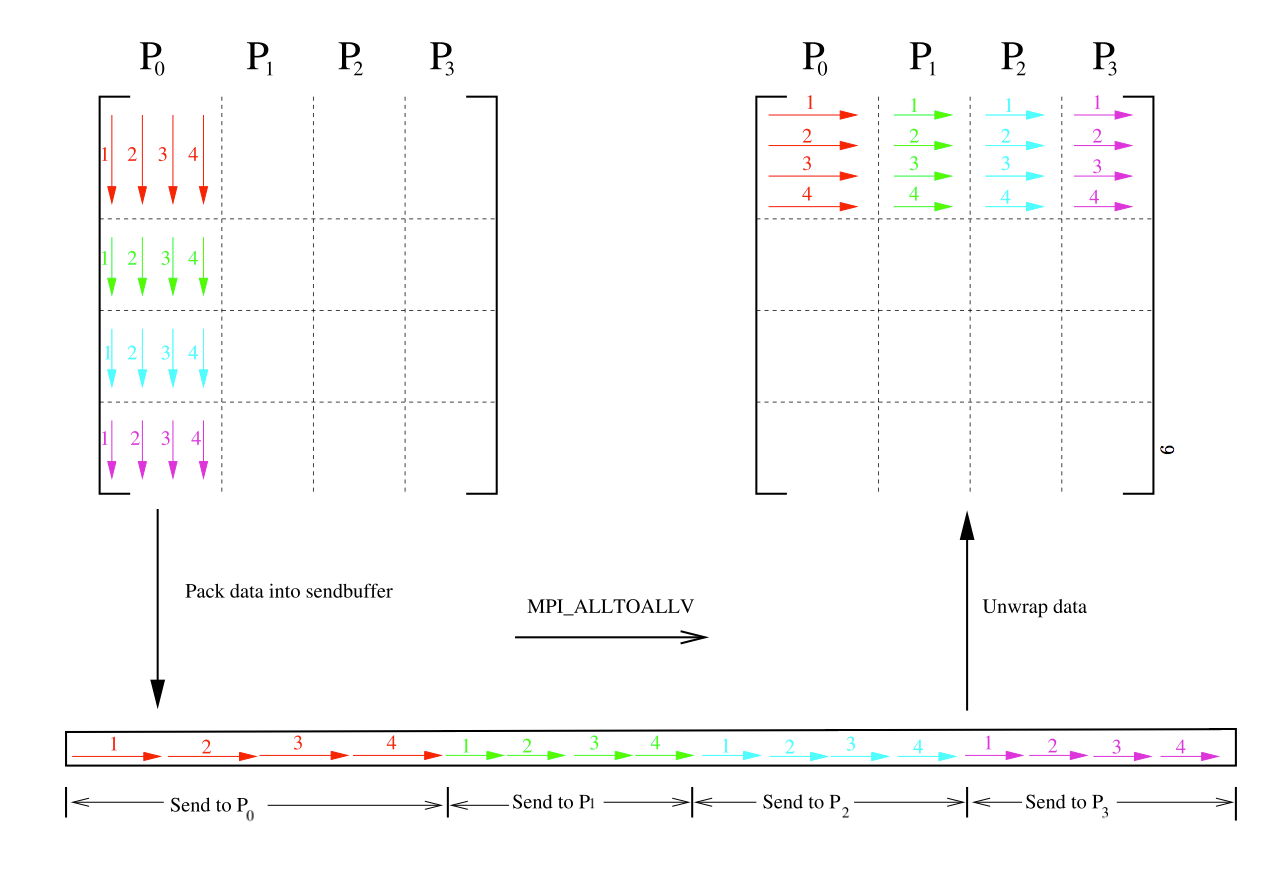
\includegraphics[width=0.8\textwidth]{transpose}
	\caption{Transpose operation through MPI\_Alltoallv}
	\label{fig:transpose}
\end{figure}

\subsection{The error computation in parallel and and results}
At computation of error there is also some need for paralellization. Generation of the problem's exact solution is done for each process', and the exact solution can therefore be compared with the solution found on each process. I here took advantage of our professor's common files, and blaslapack. 

I created a matrixToVec() operation, which transforms the processes part matrix b to a vector, as well as the process' exact solution. After this, an axpy operation is performed on the solution v.s. the exact solution. This performs the following vector operation $y <- (-1.0*solutionVector) + exactVector$. This generates the relative errors for this process' solution. 

Then the maximal local error is found with blas routine idamax, which returns the element of largest magnitude. Now each process has found the max error in it's own part solution. The global max error is computed with a call of MPI\_Reduce with MPI\_MAX, which result in the maximal pointwise error.

For a time I also assembled the final solution matrix on the root process using MPI\_Gatherv. I however found that this was unnecessary, when the results from the program is available in each process, and only the pointwise error is needed for report. 

\subsection{Use of OpenMP}
To further increase the parallelization of the program OpenMP can be used. This enables the program's MPI processes to use more than one thread in it's execution. 
The main (perhaps only) use of extra threads in this program is when performing the fourier transformations.


\section{Kongull}
Kongull has 108 compute nodes, each having 2 processors. This is divided in 96 nodes using an AMD Opteron processor with 6 cores, and 12 nodes using Intel(R) Xeon(R) processors. Depending on which rack of the compute nodes are being used, the node has 24 GiB/node or 48 GiB/node. This means that each processor has at least 12 GiB of memory (create reference to https://www.hpc.ntnu.no/display/hpc/Kongull+Hardware Compute-nodes). I believe that our student projects in TMA4280 only have access to the section having 24 GB memory per node. 

To compile and run the program I have used Intel's compilers for Fortran and C, ifortran and icc. Cmake was used to perform the compilation with these compilers. This generates a build system with portability and simplicity. 
The program uses MPI, OpenMP and BLAS/Lapack. In addition support for C99 has been added for simplicty of writing code.
All of these are installed on Kongull.


\section{Verification of correctness}
To verify that the code works correctly, I have performed a convergence test. To obtain a correct error estimate an exact solution were computed. The exact solution has been entered as 
\begin{equation}
	u(x,y) = sin(\pi x) \cdot sin(2\pi x)
\end{equation}
Which satisfies the homogeneous boundary conditions $u = 0 \text{ on } \partial\Omega$. If we then evalueate $-\nabla^2 u$ which should be equal to 
\begin{equation}
	u(x,y) = 5\pi^2 \cdot sin(\pi x) \cdot sin(2\pi x)
\end{equation}
The error gained from comparison of the exact and computed solution is then used to check whether the program performs correctly.

This test has been performed with 3 nodes with 2 processors each having 6 cores. Assigned number of threads per MPI process was 6, which perhaps is not ideal, but nevertheless. The program was executed with this setup for a number of problem sizes from $n=4 8 16 ...16384$, and the errors for each problem size is compared with $h=(1 / n)^2$. This then was processed in a octave plot using loglog, resulting in the following plot \ref{fig:loglogerror} where the gradient $a = 2.0309$ is just about two. The graph is also just about completely linear. This verifies the correctness of the solution. 
\begin{figure}[htbp]
	\centering
	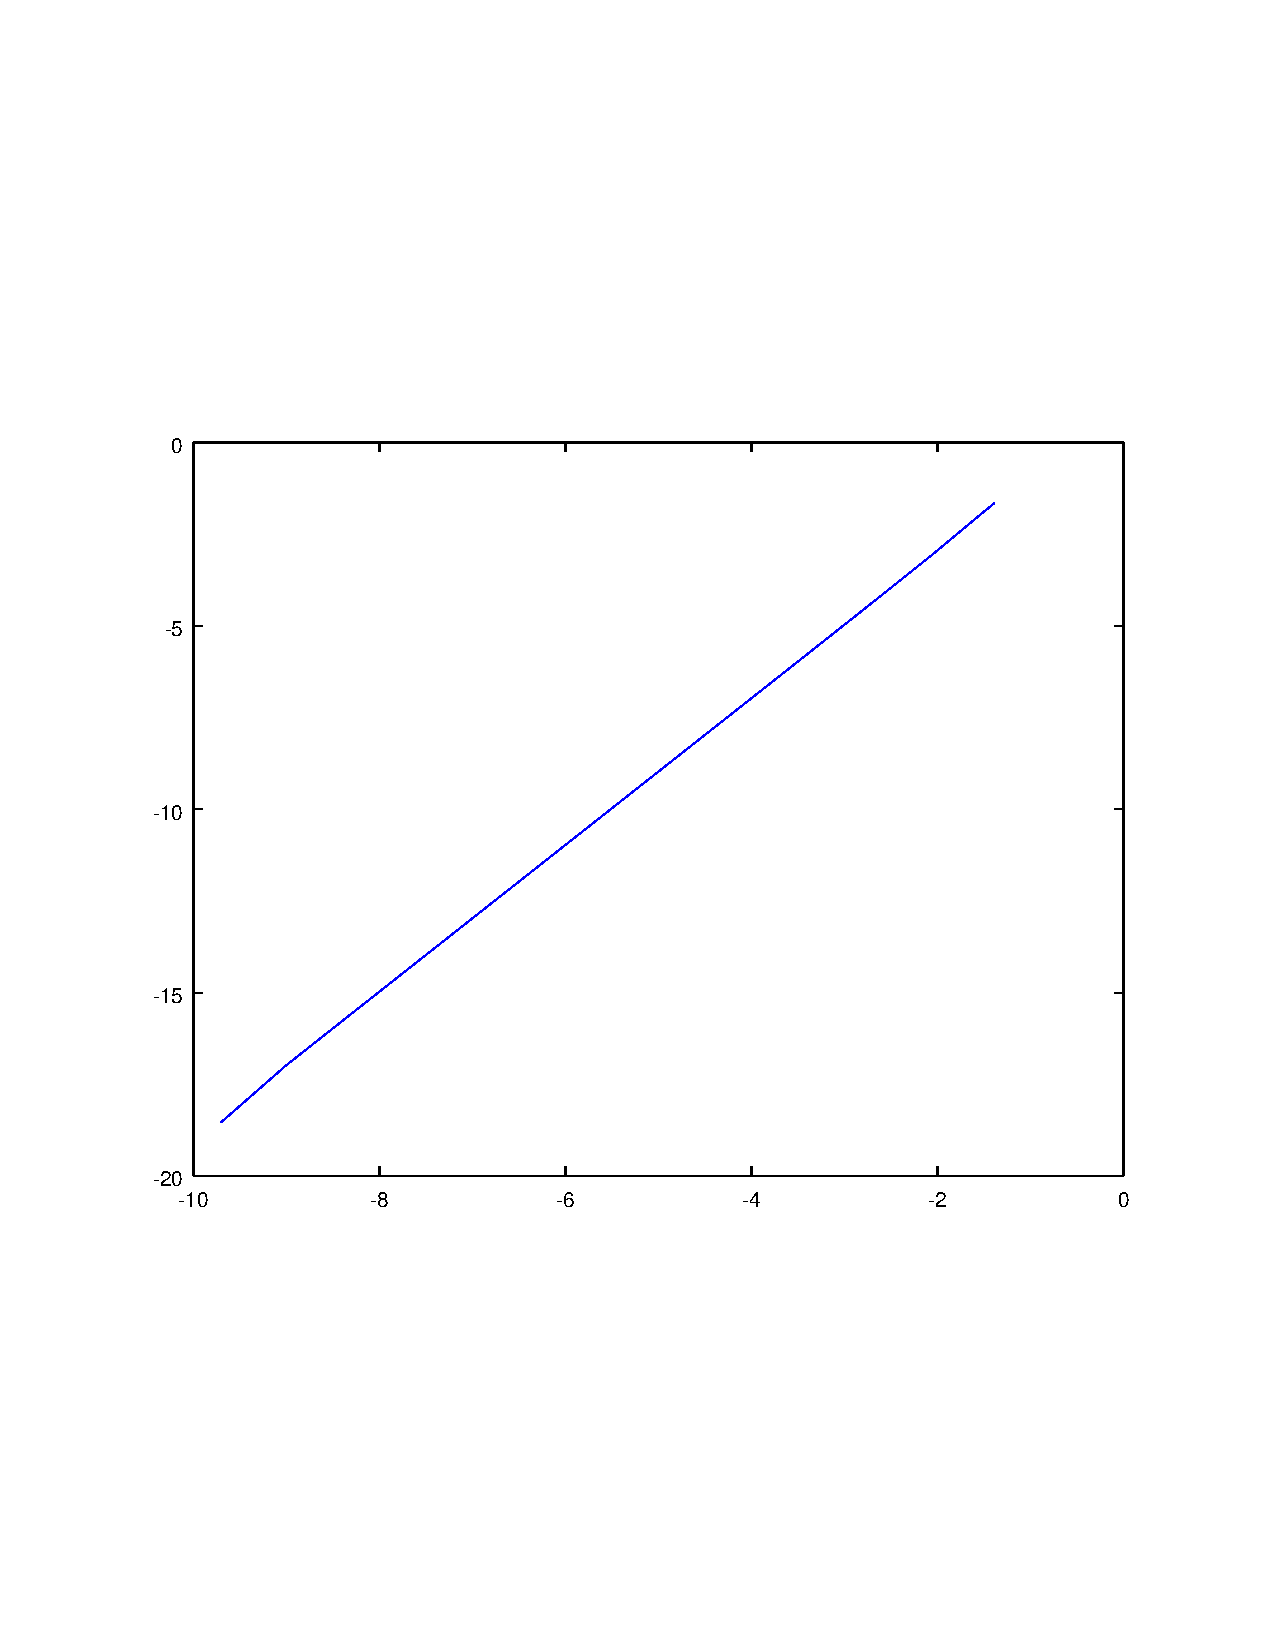
\includegraphics[width=0.8\textwidth]{loglog_error_verification}
	\caption{loglog plot of h, max pointwise error}
	\label{fig:loglogerror}
\end{figure}

\section{Hybrid v.s. Pure distributed memory model}



% \input{bakgrunn}

% \input{resultater}

% Bibliografi/referanseliste skal komme før appendiks
%\bibliography{kurs}
\bibliographystyle{plain}

% En latex-kommando for å si fra at kapitlene/seksjonene fra nå 
% av skal nummereres med store bokstaver:
\appendix

% \input{appendiks}

% Indeks for rapporten. Ta bort prosenttegn hvis du vil ha det med.
%\printindex

% Avslutter dokumentet vårt:
\end{document}

% Local Variables:
% TeX-master: "master"
% End: